4 modèles de classification seront testés : SVM, K-PPV, Régression Logistique et MLP. Pour débuter, on peut tester ces modèles avec des paramètres déterminés de façon arbitraire. Pour évaluer le score de performance, on peut utiliser la métrique qui sert à l'évaluation du concours:

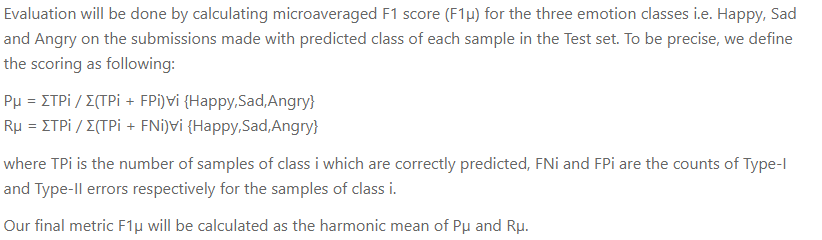
\includegraphics[width=\linewidth,height=10cm,keepaspectratio]{images/metric_concour}

Cette valeur basée sur le nombre de vrais positifs, de faux négatifs et de faux positifs de chaque classe sera calculée 3 fois avec une validation 3-plis sur nos données d'entraînement.
\begin{equation}
F1_{u} =\frac{2}{\frac{1}{P_{u}}+\frac{1}{R_{u}}}
\end{equation}

On peut tester les modèles suivants avec nos objets de compte 1 gram avec occurrence minimale de 40:
\begin{description}
\item \textbf{SVM}(Support Vector Machine): avec paramètres par défaut.
\item \textbf{KPPV} (K plus proche voisins): avec 5 voisins.
\item \textbf{Régression Logistique}: avec paramètres par défaut. (Un contre tous pour le cas multivarié)
\item \textbf{MLP} (Multi Layer Perceptron): avec 2 couches cachées de 100 neurones chaque.
\end{description}

Les résultats ainsi obtenus sont présentés dans la figure \ref{table:modeles_classification}.

% Please add the following required packages to your document preamble:
% \usepackage{multirow}
% \usepackage{longtable}
% Note: It may be necessary to compile the document several times to get a multi-page table to line up properly
\begin{longtable}[c]{cccc}
	\caption{Scores F1 de nos modèles de classification}
	\label{table:modeles_classification}\\
	\hline
	&                       & \multicolumn{2}{c}{\textbf{Score F1}}                             \\ 
	\endhead
	%
	\cline{2-4}
	\endfoot
	%
	\endlastfoot
	%
	\textbf{Vectorisation des mots}     & \textbf{Modèle}       & \textbf{Sans ajout de features} & \textbf{Avec ajout de features} \\ \hline
	\multirow{4}{*}{Word Count}         & SVM & 0,3457 & 0,3710 \\ 
	& k-PPV                 & 0,3836 & 0,4456 \\
	& Régression logistique & 0,5958 & 0,6610 \\
	& MLP                   & 0,5440 & 0,6114 \\ \hline
	\multirow{4}{*}{Word Count binaire} & SVM & 0,3223 & 0,3284 \\ 
	& k-PPV                 & 0,3727 & 0,4040 \\
	& Régression logistique & 0,6046 & 0,6797 \\
	& MLP                   & 0,5428 & 0,6141 \\ \hline
	\multirow{4}{*}{TF-IDF}             & SVM & 0,0229 & 0,0339 \\
	& k-PPV                 & 0,4440 & 0,4482 \\
	& Régression logistique & 0,5833 & 0,6552 \\
	& MLP                   & 0,5443 & 0,6115 \\ \hline
\end{longtable}

On remarque que peu importe le modèle, l'ajout d'autres features que celles de comptes augmente le score du modèle. Les 3 objets de compte semblent avoir des scores similaire d'un modèle à l'autre, on ne peut pas facilement en distinguer un qui sort du lot. Pour ce qui est des modèles de classification, le modèle de régression logistique semble mieux performer que les autres. Cela est probablement dû au fait que les autres modèles ont plus de paramètres à optimiser pour arriver à de bons résultats contrairement à la régression logistique qui en a peu (voir pas).